\chapter{KIẾN THỨC NỀN TẢNG} \label{chapter:BasedKnowledge}
Ở chương này, chúng tôi sẽ cung cấp các kiến thức được sử dụng xuyên suốt trong khóa luận này. Ở phần \ref{section:ProblemDefinition}, chúng tôi sẽ mô tả chi tiết bài toán mà chúng tôi giải quyết, bài toán Điều Hướng Thu Thập. Chúng tôi sẽ trình bày thế nào là một bài toán tối ưu hóa đa thành phần, các bài toán con, các mục tiêu đặt ra khi giải quyết bài toán này. Ở phần \ref{section:ACO}, chúng tôi sẽ trình bày các kiến thức nền tảng về giải thuật tối ưu hóa đàn kiến và biến thể MAX-MIN ACO của nó, thuật toán mà chúng tôi sử dụng làm nền tảng để phát triển nên thuật toán chúng tôi đề xuất. Bên cạnh đó chúng tôi trình bày các kiến thức cơ sở của các phương pháp chúng tôi sử dụng để thích ứng các tham số (phần \ref{section:AdaptivePheromoneRate}, \ref{section:bgCMA-ES} và \ref{section:parametersetting}) và làm giảm độ phức tạp của thuật toán (phần \ref{section:bgClusterTree}).
\section{Bài toán Điều Hướng Thu Thập}\label{section:ProblemDefinition}
\subsection{Mô tả bài toán}
Bài toán chúng tôi giải quyết ở công trình này là bài toán Điều Hướng Thu Thập (Thief Orienteering Problem, ThOP), là một biến thể của bài toán Điều Hướng (Orienteering Problem) được lấy cảm hứng từ bài toán Người Thu Thập Du Lịch (Travelling Thief Problem, TTP). TTP được đề xuất  bởi Bonyadi, Michalewicz và Barone \cite{6557681}. Đây là sự kết hợp của hai bài toán kinh điển nổi tiếng: bài toán Người Bán Hàng Du lịch (Traveling Salesman Problem, TSP) và bài toán Ba Lô (Knapsack Problem, KP). Điểm chính mà tác giả trình bày để đề xuất TTP là các thang đo của các bài toán NP-Hard kinh điển không phản ánh đúng các đặc điểm chính của các vấn đề thực tế, nên các thuật toán metaheuristics hiệu quả mà chúng ta có cho những thang đo đó không nhất thiết hiệu quả cho các vấn đề thực tế. Tác giả cho rằng sự phức tạp của các vấn đề thực tế không chỉ đến từ kích thước của chúng, mà chủ yếu là do chúng là sự kết hợp của hai hoặc nhiều vấn đề tối ưu hóa con, và vì những vấn đề con đó là tương phụ thuộc lẫn nhau. Điều này có nghĩa là việc giải quyết một vấn đề con ảnh hưởng đến chất lượng của việc giải quyết các vấn đề con khác, do đó chúng không nên được giải quyết độc lập. Trong TTP, một người thu thập phải ghé thăm mỗi thành phố trong một tập hợp gồm n thành phố (bài toán con TSP) và trong quá trình ghé thăm có thể thu thập các vật phẩm nằm ở các thành phố đó để đựng trong ba lô của mình (bài toán con KP). Tuy nhiên, khi các vật phẩm được thu thập, balo trở nên nặng hơn và người thu thập đi chậm hơn. Ba lô của người thu thập thuê, và giá phải trả là tỉ lệ với thời gian thuê. Người thu thập sau đó phải tối đa hóa tổng lợi nhuận của các vật phẩm đã thu thập và đồng thời giảm thiểu tổng thời gian của hành trình. Tác giả chỉ ra rằng giải pháp tối ưu của một trường hợp TTP có thể không bao gồm giải pháp tối ưu của bài toán con KP hoặc bài toán con TSP, chứng minh sự phụ thuộc lẫn nhau của các bài toán con trong đó.

Lấy cảm hứng từ TTP, Santos và Changas \cite{8477853} giới thiệu ở một bài toán đa thành phần mới, đó là bài toán Điều Hướng Thu Thập (ThOP), được xây dựng trên cơ sở của bài toán Điều Hướng (OP) thay vì bài toán Người Bán Hàng Du Lịch như TTP. Bài toán Điều Hướng dựa trên một trò chơi thể thao địa hình. Trong trò chơi, các đối thủ bắt đầu từ một điểm cho trước, đi qua một khu vực ghé thăm các điểm kiểm tra và phải quay lại một điểm kiểm soát trong một khoảng thời gian nhất định. Họ có một bản đồ của khu vực và phải tự quyết định tuyến đường qua các điểm kiểm tra dựa trên kỹ năng định hình và cấp độ thể dục của họ. Trong OP, mỗi điểm kiểm tra có điểm số, vì vậy mục tiêu là tìm ra tuyến đường tối đa hóa tổng điểm số, tức là tổng số điểm của các điểm kiểm tra đã ghé thăm là tối đa. Trong biến thể ThOP, một đối thủ hay chúng tôi gọi là người thu thập không ghi điểm chỉ bằng cách ghé thăm các điểm trên bản đồ, mà phải thu thập các vật phẩm tại các điểm và mang theo chúng đến điểm kết thúc. Mỗi đối thủ có một ba lô với sức chứa giới hạn cho các vật phẩm được thu thập. Hơn nữa, tốc độ của người thu thập bị ảnh hưởng trực tiếp bởi trọng lượng của ba lô. Như ở bài toán TTP, khi các vật phẩm được thu thập, ba lô sẽ nặng dần, và tốc độ của người thu thập sẽ giảm xuống. Gọi $v_{min}$, $v_{max}$ là tốc độ tối thiểu và tốc độ tối đa mà người thu thập di chuyển tương ứng khi ba lô đạt sức chứa giới hạn $W$ hoặc ba lô rỗng. Tốc độ di chuyển $v$ của người thu thập với ba lô có sức nặng $w$, $0 \leq w \leq W$ được tính bằng $v = v_{max} - w \cdot(v_{max} - v_{min})/W$. Lưu ý rằng giá trị $(v_{max} - v_{min})/W$ là hằng số và thể hiện độ giảm của tốc độ với một đơn vị cân nặng của ba lô.

Mục tiêu của ThOP là cung cấp một đường đi từ thành phố bắt đầu 1 đến thành phố kết thúc n, cũng như một tập các vật phẩm được chọn từ các thành phố đã ghé thăm trong suốt hành trình để tối đa hóa tổng lợi nhuận đã lấy, đồng thời đảm bảo rằng sức chứa của balo không vượt quá sức chứa giới hạn $W$ và tổng thời gian di chuyển của người thu thập nằm trong giới hạn thời gian $T$. Người thu thập không cần phải ghé thăm tất cả các thành phố.

\begin{figure}[ht!]
    \centering
    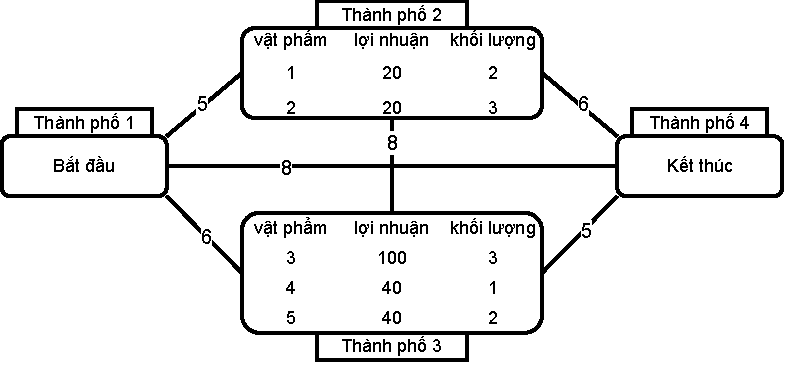
\includegraphics[width=\textwidth]{Figures/ThOP-instance.pdf}
    \caption[Minh họa một ví dụ của bài toán Điều Hướng Thu Thập.]{Minh họa một ví dụ của bài toán Điều Hướng Thu Thập bao gồm 4 thành phố, 5 vật phẩm.}
    \label{fig:ThOPinstance}
\end{figure}

Để hiểu rõ bài toán Điều Hướng Thu Thập ThOP, chúng tôi minh họa trong hình \ref{fig:ThOPinstance} một ví dụ nhỏ của một trường hợp ThOP liên quan đến 4 thành phố và 5 vật phẩm. Lưu ý rằng không có vật phẩm nào ở thành phố bắt đầu (1) và thành phố kết thúc (4), các số vật phẩm có trọng lượng và lợi nhuận khác nhau được phân phối ở các thành phố khác (2 và 3). Các khoảng cách từ mỗi cặp thành phố được cho trong các cạnh. Dưới đây, chúng tôi trình bày chi tiết một số lời giải cho trường hợp này. Chúng tôi đặt các ràng buộc của ví dụ này như sau: $v_{min} = 0.1$, $v_{max} = 1.0$, $W = 3$ và $T = 75$.

Chúng tôi biểu diễn một lời giải cho bài toán ThOP dưới dạng hai phần ($\pi$, $z$). Phần đầu tiên bao gồm tuyến đường di chuyển của người thu thập $\pi = \langle 1, \pi_2, \pi_3, ..., \\\pi_k, n \rangle$, một véc tơ chứa danh sách thành phố đã ghé thăm theo thứ tự di chuyển. Lưu ý rằng thành phố đầu tiên và cuối cùng được cố định cho mọi lời giải hợp lệ. Phần thứ hai là chiến lược thu thập vật phẩm $z = \langle z_1, z_2, . . . , z_m \rangle$, một véc tơ nhị phân đại diện cho trạng thái của các vật phẩm ($z_i = 1$ nếu vật phẩm i được lấy, và 0 nếu ngược lại). Theo biểu diễn này, hãy xem xét các lời giải ThOP sau cho trường hợp đã mô tả ở trên:
\begin{itemize}
    \item $(\langle1,2,3,4\rangle,\langle1,0,0,1,0\rangle)$: là một lời giải hợp lệ với tổng lợi nhuận là $20+40=60$. Tổng khối lượng các vật phẩm được thu thập là 3 và thời gian di chuyển là 75, thỏa mãn cả hai ràng buộc giới hạn sức chứa ba lô $W$ và thời gian di chuyển $T$. Tổng thời gian di chuyển được tính như sau:
    \begin{itemize}
        \item di chuyển từ thành phố bắt đầu đến thành phố thứ 2 với tốc độ tối đa: thời gian di chuyển là $d_{12}/v_{max}=5/1.0=5$ 
    	\item tại thành phố thứ 2, người thu thập lấy vật phẩm 1: vận tốc giảm xuống $v=1.0-2\times(1.0-0.1)/3=0.4$ 
    	\item di chuyển từ thành phố thứ 2 sang thành phố thứ 3: tổng thời gian di chuyển là $5+d_{23}/v=5+8/0.4=5+20=25$ 
    	\item tại thành phố thứ 3, vật phẩm thứ 4 được lấy: vận tốc giảm xuống $v=1.0-3\times(1.0-0.1)/3=0.1$ 
    	\item di chuyển từ thành phố thứ 3 đến thành phố kết thúc 4: tổng thời gian di chuyển là $5+20+d_{34}/v=5+20+5/0.1=5+20+50=75$ 
    \end{itemize}
    \item $(\langle1,3,2,4\rangle,\langle1,0,0,1,0\rangle)$: là một lời giải không hợp lệ. Mặc dù chiến lược thu thập với lời giải ơ trên nhưng tổng thời gian di chuyển (83.43) vượt quá ràng buộc thời gian:
    \begin{itemize}
        \item di chuyển từ thành phố bắt đầu đến thành phố thứ 3 với tốc độ tối đa: thời gian di chuyển là $d_{13}/v_{max}=6/1.0=6$ 
    	\item tại thành phố thứ 3, người thu thập lấy vật phẩm 4: vận tốc giảm xuống $v=1.0-1\times(1.0-0.1)/3=0.7$ 
    	\item di chuyển từ thành phố thứ 3 sang thành phố thứ 2: tổng thời gian di chuyển là $6+d_{32}/v=6+8/0.7=6+11.43=17.43$ 
    	\item tại thành phố thứ 2, vật phẩm thứ 1 được lấy: vận tốc giảm xuống $v=1.0-3\times(1.0-0.1)/3=0.1$ 
    	\item di chuyển từ thành phố thứ 2 đến thành phố kết thúc 4: tổng thời gian di chuyển là $6+17.43+d_{24}/v=6+17.43+6/0.1=83.43$ 
    \end{itemize}
	\item $(\langle1,3,4\rangle,\langle0,0,1,0,0\rangle)$: là một lời giải tối ưu cho trường hợp ví dụ này với tổng lợi nhuận là 100. Tổng khối lượng ba lô là $3\leq W$ và tổng thời gian di chuyển là $56 \leq T$:
    \begin{itemize}
        \item di chuyển từ thành phố bắt đầu đến thành phố thứ 3 với tốc độ tối đa: thời gian di chuyển là $d_{13}/v_{max}=6/1.0=6$ 
        \item tại thành phố thứ 3, người thu thập lấy vật phẩm 3: vận tốc giảm xuống $v=1.0-3\times(1.0-0.1)/3=0.1$ 
        \item di chuyển từ thành phố thứ 3 đến thành phố kết thúc 4: tổng thời gian di chuyển là $6+d_{34}/v=6+5/0.1=6+50=56$ 
    \end{itemize}
\end{itemize}

Lưu ý rằng chiến lược thu thập của lời giải tối ưu cho trường hợp ví dụ giống như lời giải tối ưu cho bài toán con Ba Lô. Tuy nhiên, không phải lúc nào người thu thập cũng có chiến lược thu thập vật phẩm tốt nhất giống với lời giải tốt ưu cho bài toán con Ba Lô trong giới hạn thời gian $T$. Để minh họa điều này, hãy xem xét một giới hạn thời gian chặt chẽ hơn là 20 với ví dụ trước đó. Trong trường hợp này, lời giải  tối ưu sẽ là $(\langle1, 3, 4\rangle, \langle0, 0, 0, 1, 1\rangle)$, có tổng lợi nhuận là 80 và tổng thời gian di chuyển là 18.5.
\subsection{Biểu diễn toán học}
Ở phần này chúng tôi trình bày mô hình bài toán Điều Hướng Thu Thập dưới dạng công thức toán học không tuyến tính. Với bài toán ThOP, chúng ta có một tập hợp gồm $n$ thành phố: 1 là thành phố bắt đầu, $n$ là thành phố kết thúc, và các thành phố còn lại $(2, . . . , n - 1)$ là các thành phố trung gian. Tại mỗi thành phố trung gian có một hoặc nhiều vật phẩm, và đối với mỗi vật phẩm $i$, chúng ta có lợi nhuận $p_i$ và trọng lượng $w_i$ của nó. Chúng ta cũng được cho biết giới hạn sức chứa $W$ của ba lô, giới hạn thời gian di chuyển $T$ để đến thành phố kết thúc, tốc độ tối đa và tối thiểu của người thu thập lần lượt là $v_{max}$ và $v_{min}$, và khoảng cách $d_{ij}$ giữa mọi cặp điểm $i$ và $j$. Mục tiêu là tìm ra một tuyến đường di chuyển từ thành phố bắt đầu đến thành phố kết thúc, vật phẩm được chọn cẩn thận vào ba lô tại các thành phố trung gian đã ghé thăm, để tối đa hóa tổng lợi nhuận của ba lô, với ràng buộc không vượt quá khả năng sức chứa của ba lô $W$ và tổng thời gian di chuyển nằm trong giới hạn thời gian $T$.

Công thức toán học sau bao gồm tất cả các đặc tính của bài toán. Để có thể mô tả rõ ràng, các tác giả cho $S_i$ là tập các vật phẩm được đặt tại thành phố $i$. Với mỗi $s\subseteq S_i$, $w_i^s$ biểu diễn tổng khối lượng của các vật phẩm trong $s$ và $p_i^s$ là tổng lợi nhuận trong tập con này. Hơn nữa, hằng số $\nu=(v_{max} - v_{min})/W$ đại diện cho độ mất mát vận tốc cho mỗi đơn vị cân nặng bên trong ba lô, và $M'$ và $M''$ là hai hằng số đủ lớn. Các biến quyết định bao gồm:
\begin{itemize}
    \item $x_{ij}^s$: biến nhị phân nhận giá trị 1 nếu người thu thập đi qua cạnh $(i, j)$ sau khi thu thập các vật phẩm trong tập con $s\subseteq S_i$ và ngược lại nhận giá trị 0.
    \item $q_i$: cho biết khối lượng của ba lô sau khi thu thập các vật phẩm tại thành phố $i$.
    \item $t_i$: cho biết thời gian người thu thập tới thành phố $i$.
\end{itemize}

\begin{equation}\label{eq:thop1}
    \max \sum_{i=1}^{n-1} \sum_{j=2}^n \sum_{s \subseteq S_i} p_i^s \cdot x_{i j}^s
\end{equation}

\begin{equation}\label{eq:thop2}
    \sum_{j=2}^n x_{1 j}^{\varnothing}=1
\end{equation}

\begin{equation}\label{eq:thop3}
    \sum_{i=1}^{n-1} \sum_{s \subseteq S_i} x_{i n}^s=1
\end{equation}

\begin{equation}\label{eq:thop4}
    \sum_{i=1}^{n-1} \sum_{s \subseteq S_i} x_{i j}^s-\sum_{i=2}^n \sum_{s \subseteq S_j} x_{j i}^s=0 \quad \forall j=2 . . n-1
\end{equation}

\begin{equation}\label{eq:thop5}
    q_j \geq q_i +\sum_{j^{\prime}=2}^n \sum_{s \subseteq S_j} w_j^s \cdot x_{j j^{\prime}}^s-M^{\prime} \cdot\left(1-\sum_{s \subseteq S_i} x_{i j}^s\right) \quad \forall i=1 .. n, \forall j=1..n 
\end{equation}

\begin{equation}\label{eq:thop6}
    t_j \geq t_i+ \frac{d_{i j}}{v_{\max }-\nu \cdot q_i} -M^{\prime \prime} \cdot\left(1-\sum_{s \subseteq S_i} x_{i j}^s\right) \quad \forall i=1 .. n, \forall j=1..n 
\end{equation}

\begin{equation}\label{eq:thop7}
    x_{i j}^s \in\{0,1\} \quad \forall i=1 .. n,\forall j=1 .. n
\end{equation}

\begin{equation}\label{eq:thop8}
    0 \leq q_i \leq W \quad \forall s \subseteq S_i
\end{equation}

\begin{equation}\label{eq:thop9}
    0 \leq t_i \leq T \quad \forall i=1 .. n, \forall i=1 .. n
\end{equation}

Mục tiêu (\ref{eq:thop1}) là tối đa hóa tổng lợi nhuận của các vật phẩm thu thập. Người thu thập phải bắt đầu tại thành phố 1 mang theo một ba lô rỗng (\ref{eq:thop2}) và đến thành phố $n$ (\ref{eq:thop3}), ghé thăm bất kỳ thành phố nào trung gian trên đường (\ref{eq:thop4}). Sau khi ghé thăm một thành phố, người thu thập phải rời đi sau khi thu thập một phần của các vật phẩm của thành phố đó (\ref{eq:thop4}), điều này làm tăng trọng lượng của balo (\ref{eq:thop5}) và giảm tốc độ di chuyển tương ứng, ảnh hưởng đến thời gian để đến thành phố tiếp theo (\ref{eq:thop6}). Trọng lượng của ba lô và tổng thời gian đi bộ phải luôn nằm trong các giới hạn đã cho (\ref{eq:thop8})-(\ref{eq:thop9}).

Lưu ý rằng bộ ràng buộc này là đủ để tránh các chu kỳ con trên đường đi, vì (\ref{eq:thop4}) đảm bảo luồng đường đi và (\ref{eq:thop5})-(\ref{eq:thop6}) đảm bảo rằng trọng lượng của balo và thời gian của đường đi tăng dần theo chiều dài của đường đi.

Mặc dù đầy đủ, nhưng công thức hiện tại công thức không thể được sử dụng để giải quyết vấn đề do sự phức tạp của nó: số lượng biến là số mũ của số lượng vật phẩm của một thành phố cụ thể bởi vì số lượng tập con có thể xảy ra; và ràng buộc (\ref{eq:thop6}) là phi tuyến tính, khoảng cách được chia cho một biến liên tục. Các thuật toán để giải quyết bài toán này hầu hết là các thuật toán heuristics.

\section{Giải thuật tối ưu hóa đàn kiến cho bài toán ThOP}\label{section:ACO}

Ở phần này chúng tôi sẽ trình bày một thuật toán cho bài toán ThOP được dựa trên giải thuật tối ưu hóa đàn kiến được gọi là ACO++. Thuật toán này sử dụng một biết thể của giải thuật đàn kiến là MAX-MIN Ant System \cite{STUTZLE2000889} để xử lý bài toán con OP và một thuật toán heuristic cho bài toán con KP. Thuật toán ACO++ thể hiện kết quả vượt trội so với các thuật toán khác tại thời điểm được công bố và là thuật toán cơ sở để chúng tôi phát triển lên thuật toán SAAS kế thừa các ưu điểm và khắc phục các nhược điểm của ACO++. Chúng tôi sẽ mô tả chi tiết thuật toán ACO++ ở phần \ref{section:ACO++} và thuật toán thu thập heuristic ở phần \ref{section:PackingHeuristic}. Ở phần \ref{section:ACO++Sensitive} chúng tôi sẽ trình bày thực nghiệm của chúng tôi về độ nhạy của thuật toán ACO++ với các siêu tham số của nó.

\subsection{Thuật toán tối ưu hóa đàn kiến} \label{section:ACO++}
Thuật toán ACO++ của Changas và Wagner là một hướng tiếp cận heuristic cho bài toán ThOP. Nó được dựa trên công trình của Wagner cho bài toán TTP. Thuật toán ACO++ được dựa trên biến thể thuật toán tối ưu hóa đàn kiến MAX-MIN Ant System (MMAS) để giải bài toán con tìm tuyến đường của ThOP, trong khi đó một thuật toán heuristic khác đảm nhận việc thu thập các vật phẩm.

Các thuật toán dựa trên thuật toán tối ưu hóa đàn kiến bao gồm một lớp quan trọng của các kỹ thuật tìm kiếm theo xác suất được lấy cảm hứng từ hành vi của kiến thật. Những thuật toán này đã chứng minh được tính hiệu quả trong việc giải quyết nhiều bài toán tổ hợp \cite{DORIGO2005243}. Ý tưởng cơ bản của thuật toán tối ưu hóa đàn kiến là đàn kiến tạo các giải pháp cho một vấn đề cụ thể bằng cách thực hiện các bước đi trên một đồ thị gọi là đồ thị xây dựng. Những bước đi này được ảnh hưởng bởi giá trị pheromone được lưu trữ dọc theo các cạnh của đồ thị. Trong quá trình tối ưu hóa, giá trị pheromone được cập nhật dựa trên các giải pháp tốt được tìm thấy trong quá trình tối ưu hóa, điều này sau đó sẽ dẫn dắt đàn kiến đến các giải pháp tốt hơn trong các lần lặp tiếp theo của thuật toán.

Biến thể MMAS của giải thuật đàn kiến được thiết kế để cái thiện hiệu suất của thuật toán gốc. Đặc điểm thứ nhất, nó tận dụng mạnh mẽ các đường đi tốt nhất được tìm thấy: chỉ có một trong hai con kiến được dùng để cập nhật pheromone, đó là kiến đã tạo ra đường đi tốt nhất trong vòng lặp hiện tại, hoặc kiến tốt nhất cho tất cả vòng lặp. Thật không may, chiến lược như vậy có thể dẫn đến tình trạng đình trệ trong đó tất cả các kiến đi theo cùng một đường đi, do sự tăng quá mức của đường mùi trên các cung của một đường đi tốt, mặc dù không tối ưu. Để chống lại hiệu ứng này, đặc điểm thứ hai được giới thiệu bởi MMAS là giới hạn khoảng giá trị đường mùi có thể đạt được trong khoảng $[\tau_{min},\tau_{max}]$. Đặc điểm thứ ba, các đường mùi được khởi tạo với giá trị nồng độ pheromone tối đa cùng với một tỷ lệ bay hơi pheromone nhỏ, làm tăng cường sự khám phá của các đường đi ở giai đoạn đầu quá trình tìm kiếm. Cuối cùng, trong MMAS, nồng độ pheromone trên các đường đi được khởi tạo lại mỗi khi thuật toán có tình trạng đình trệ hoặc khi không có đường đi cải thiện nào được tạo ra trong một số lượng vòng lặp liên tiếp nhất định.

Ở thuật toán ACO++ cho ThOP, để xây dựng các tuyến đường một đàn kiến gồm $n_{ants}$ kiến được đặt ở thành phố xuất phát. Với mỗi bước đàn kiến đi tới một thành phố trong tập các thành phố chưa được thăm (ký hiệu là $V_{unvisited}$) dựa trên xác suất di chuyển được tính bằng công thức \ref{eq:ACOtransProb}. Xác suất di chuyển được ảnh bởi vết pheromone $\tau_{i k}$ và thông tin heuristic $\eta_{i j}$ (thường được chọn là nghịch đảo của khoảng cách của cạnh nối thành phố $i$ và thành phố $j$). Độ quan trọng của vết pheromone và thông tin heuristic được quyết định với 2 hệ số $\alpha$ và $\beta$. Quá trình xây dựng các tuyến đường dừng lại khi tất cả các con kiến dừng chân tới thành phố kết thúc.

\begin{equation}\label{eq:ACOtransProb}
      p\left(v_i \rightarrow v_j\right)=\frac{\tau_{i j}^\alpha \cdot \eta_{i j}^\beta}{\sum_{v_k \in V_{\text {unvisited }}} \tau_{i k}^\alpha \cdot \eta_{i k}^\beta} \text { for all } v_j \in V_{\text {unvisited }}.
\end{equation}

Vết pheromone được trình bày ở công thức \ref{eq:ACOpheromone}, sẽ phải bay hơi một lượng tương ứng với $\rho$ qua từng lần lặp của thuật toán. Sau đó, lời giả của con kiến có lời giải tốt nhất trong lần lặp hiện tại được dùng để cập nhật pheromone, được ký hiệu là $\Delta\tau_{i j}$.

\begin{equation}\label{eq:ACOpheromone}
    \begin{split}
        \tau_{i j} &\gets (1-\rho)\cdot\tau_{i j}+x_{i j} \cdot \delta \cdot \Delta\tau_{i j} \text { for all } v_i, v_j \in V ,\\
        x_{i j} &=\left\{\begin{array}{l}1 \text { nếu } \text{cạnh}_{ij} \text { nằm trên tuyến đường của con kiến có lời giải tốt nhất, } \\ 0 \text { ngược lại. }\end{array}\right. \\
        \delta  &= 1 \text { là hệ số cập nhật pheromone. }
    \end{split}
\end{equation}

Trong giải thuật \ref{algo:bgACO++}, chúng tôi trình bày mã giả đơn giản của ACO++. Ở đầu (dòng \ref{bgACO++:step1}), lời giải tốt nhất được tìm thấy (tuyến đường đi và chiến lược thu thập) được khởi tạo là một lời giải rỗng. Thuật toán thực hiện chu kỳ lặp của mình (dòng \ref{bgACO++:step2} đến \ref{bgACO++:step18}) đến khi điều kiện dừng chưa được thỏa mãn. Tại dòng \ref{bgACO++:step3}, mỗi con kiến tạo một đường đi cho người thu thập, sau đó chiến lược thu thập được tạo ra (dòng \ref{bgACO++:step4} và \ref{bgACO++:step5}). Sau đó ACO++ áp dụng một số thuật toán heuristic tìm kiếm cục bộ kinh điển: 2-OPT, 2:5-OPT và 3-OPT \cite{Crama1995} để cải thiện chí phí khoảng cách. Nếu bất kỳ tìm kiếm cục bộ nào được kích hoạt trong thuật toán (dòng \ref{bgACO++:step6}), thủ tục tìm kiếm cục bộ đó sẽ được thực hiện trên mỗi tuyến đường đi $\pi$, do đó tạo ra các tuyến đường đi mới $\pi'$ (dòng \ref{bgACO++:step7}), có thể tốt hơn $\pi$ khi so với chi phí khoảng cách. Trong bước tiếp theo, một chiến lược thu thập $z'$ được tạo từ $\pi'$ (dòng \ref{bgACO++:step8}). Nếu $z'$ tốt hơn $z$ (dòng \ref{bgACO++:step9}), $pi$ và $z$ được thay thế bằng $\pi'$ và $z'$ (dòng \ref{bgACO++:step10}). Tại dòng \ref{bgACO++:step13} đến \ref{bgACO++:step15}, thuật toán cập nhật lời giải tốt nhất. Lưu ý rằng, để đạt được các đường đi hiệu quả hơn, thuật toán loại bỏ từ tuyến đường đi $\pi$ tất cả các thành phố mà không có vật phẩm nào được lấy (dòng \ref{bgACO++:step14}). Sau khi xem xét tất cả các đường đi, vết pheromone được cập nhật dựa trên chất lượng của các lời giải (dòng \ref{bgACO++:step17}). Cuối cùng, lời giải tốt nhất được tìm thấy được trả về.

\begin{algorithm}
\caption{Thuật toán ACO++ cho bài toán ThOP}
\label{algo:bgACO++}
\algorithmfootnote{$\zeta(\pi)$ bỏ đi các thành phố không có vật phẩm được thu tập từ chiến lược thu thập $z$ từ $\pi$.} 
$\pi^{best} \leftarrow \varnothing , z^{best} \leftarrow \varnothing$\; \label{bgACO++:step1} 
\Repeat{điều kiện dừng được thỏa mãn}{ \label{bgACO++:step2}
    $\Pi \leftarrow$ xây dựng các tuyến đường bằng đàn kiến \; \label{bgACO++:step3}
    \ForEach{chu trình TSP $\pi \in \Pi$}{ \label{bgACO++:step4}
        $z \leftarrow$ xây dựng chiến lược thu thập từ $\pi$ bằng $Pack(\pi, ptries)$ \; \label{bgACO++:step5}
        \If{tìm kiếm địa phương được bật}{ \label{bgACO++:step6}
            $\pi' \leftarrow$ thực hiện tìm kiếm địa phương trên truyền đường $\pi$\; \label{bgACO++:step7}
            $z' \leftarrow$ xây dựng chiến lược thu thập từ $\pi'$ bằng $Pack(\pi', ptries)$ \; \label{bgACO++:step8}
            \If{giá trị lợi nhuận của $z'$ lớn hơn giá trị lợi nhuận của $z$ }{ \label{bgACO++:step9}
                $\pi \leftarrow \pi', z \leftarrow z'$ \label{bgACO++:step10}
            } \label{bgACO++:step11}
        } \label{bgACO++:step12}
        \If{giá trị lợi nhuận của $z$ lớn hơn giá trị lợi nhuận của $z^{best}$}{ \label{bgACO++:step13}
            $\pi^{best} \leftarrow \zeta(\pi), z^{best} \leftarrow z$ \label{bgACO++:step14}
        } \label{bgACO++:step15}
    } \label{bgACO++:step16}
    cập nhật số liệu của ACO và dấu vết của pheromone\; \label{bgACO++:step17}
} \label{bgACO++:step18}
\Return{$\pi^{best}, z^{best}$} \label{bgACO++:step19}
\end{algorithm}

\subsection{Thuật toán thu thập heuristic} \label{section:PackingHeuristic}

Trong giải thuật \ref{algo:bgPack}, chúng tôi trình bày thuật toán thu thập heuristic, của Changas và Wagner đề xuất \cite{CHAGAS2020708}, để xây dựng một chiến lược thu thập từ một tuyến đường đi cố định. Lưu ý rằng ngay cả khi đường đi của người thu thập được giữ cố định, việc tìm một chiến lược thu thập tối ưu là bài toán NP-khó. 

\begin{algorithm}
\caption{Thuật toán thu thập: $Pack(\pi, ptries)$}
\label{algo:bgPack}
$z \leftarrow \varnothing , try \leftarrow 1$\;
\Repeat{try > ptries}{ \label{algoPackingHeuristic:step2}
    chọn một số thực cho mỗi tham số $\theta$, $\delta$, và $\gamma$ từ một phân phối chuẩn trong khoảng $[0, 1]$, để $\theta + \delta + \gamma = 1$\; \label{algoPackingHeuristic:step3}
    \ForEach{$i \leftarrow 1$ \textbf{to} m }{ \label{algoPackingHeuristic:step4}
        tính giá trị điểm số $s_i$ cho vật phẩm $i$\; \label{algoPackingHeuristic:step5}
    }
    $z \leftarrow \varnothing$ \;
    \For{$j\leftarrow 1$ \textbf{to} m}{  \label{algoPackingHeuristic:step7}
        $i \leftarrow$ chọn vật phẩm có điểm số cao thứ $j$ \;
        $z' \leftarrow z' \cup \{i\}$ \;
        \uIf{trọng lượng của $z'$ lớn hơn $W$}{ \label{algoPackingHeuristic:step10}
            $z' \leftarrow z' \backslash \{i\}$ \; 
        }
        \Else{
            $t \leftarrow$ tính thời gian cần thiết để thu thập theo chiến lược $z'$ bằng cách đi qua các thành phố trong hành trình $\pi$ \; \label{algoPackingHeuristic:step12}
            \If{nếu thời gian $t$ lâu hơn ràng buộc $T$}{\label{algoPackingHeuristic:step13.5}
                $z' \leftarrow z' \backslash \{i\}$ \;
            }
        }
    }\label{algoPackingHeuristic:step13}
    \If{giá trị lợi nhuận của $z'$ lớn hơn giá trị lợi nhuận của $z$}{ \label{algoPackingHeuristic:step14}
        $z \leftarrow z'$\; \label{algoPackingHeuristic:step14.5}
    }
    $try \leftarrow try + 1$\;
}\label{algoPackingHeuristic:step16}
\Return{$z$}\label{algoPackingHeuristic:step17}
\end{algorithm}

Thuật toán thu thập heuristic này  cố gắng tìm một chiến lược thu thập tốt từ nhiều thử nghiệm cho cùng một tuyến đường đi $\pi$. Số lượng thử nghiệm được xác định bởi $ptries$. Mỗi lần thử nghiệm được mô tả từ dòng \ref{algoPackingHeuristic:step2} đến \ref{algoPackingHeuristic:step16}. Ở đầu mỗi lần thử nghiệm (dòng \ref{algoPackingHeuristic:step3}), thuật toán chọn đồng đều ba giá trị ngẫu nhiên ($\theta$, $\delta$, và $\gamma$) giữa 0 và 1, sau đó chuẩn hóa chúng sao cho tổng của chúng bằng 1. Các giá trị này được sử dụng để tính điểm cho mỗi vật phẩm $i\in \{1,...,m\}$ (dòng \ref{algoPackingHeuristic:step4} đến \ref{algoPackingHeuristic:step5}), trong đó $\theta$, $\delta$, và $\gamma$ xác định, tương ứng, các số mũ được áp dụng cho lợi nhuận $p_i$, trọng lượng $w_i$, và khoảng cách $d_i$ để quản lý tác động của chúng. Khoảng cách $d_i$ được tính toán theo tuyến đường đi $\pi$ bằng cách tính tổng tất cả các khoảng cách từ thành phố chứa vật phẩm $i$ đến thành phố cuối cùng. Công thức \ref{eq:itemScore} cho thấy cách điểm của vật phẩm $i$ được tính.

\begin{equation}\label{eq:itemScore}
    s_i = \frac{p_i^\theta}{w_i^\delta \cdot d_i^\gamma}.
\end{equation}

Lưu ý rằng mỗi điểm số $s_i$ tích hợp một sự cân đối giữa khoảng cách mà vật phẩm i phải được mang qua, trọng lượng của nó và lợi nhuận của nó. Công thức \ref{eq:itemScore} dựa trên thuật toán heuristic PackIterative đã được phát triển cho TTP \cite{10.1145/2739480.2754716}. Tuy nhiên, khác với \cite{10.1145/2739480.2754716} thuật toán xem xét một số mũ cho tham số của khoảng cách để xét tầm quan trọng của ảnh hưởng của nó. Hơn nữa, các giá trị của tất cả các số mũ đều được chọn ngẫu nhiên từ 0 đến 1 cho mỗi lần thử nghiệm (và sau đó được chuẩn hóa) để tìm kiếm không gian cho các chiến lược thu thập tham lam.

Sau khi tính toán điểm cho tất cả các vật phẩm, thuật toán sử dụng giá trị của chúng để xác định ưu tiên của mỗi vật phẩm trong chiến lược thu thập. Điểm số của một vật phẩm càng lớn, ưu tiên của nó càng cao. Giữa các dòng \ref{algoPackingHeuristic:step7} và \ref{algoPackingHeuristic:step13}, chúng tôi tạo chiến lược thu thập cho lần thử nghiệm hiện tại bằng cách xem xét các vật phẩm theo ưu tiên của chúng. Nếu một vật phẩm vi phạm ràng buộc của bài toán ThOP (dòng \ref{algoPackingHeuristic:step10} và \ref{algoPackingHeuristic:step13.5}), nó sẽ không được chọn. Lưu ý rằng thuật toán tính thời gian di chuyển (dòng \ref{algoPackingHeuristic:step12}) từ các thành phố được liệt kê trên đường đi $\pi$, nhưng thuật toán bỏ qua những thành phố nơi không có vật phẩm nào được chọn. Sau khi hoàn thành chiến lược thu thập của lần thử nghiệm hiện tại, tổng lợi nhuận của nó được so sánh với chiến lược thu thập tốt nhất cho đến nay (dòng \ref{algoPackingHeuristic:step14}), sau đó cập nhật chiến lược thu thập tốt nhất cho đến nay (dòng \ref{algoPackingHeuristic:step14.5}). Ở cuối tất cả các lần thử nghiệm, chiến lược thu thập tốt nhất được tìm thấy được trả về (\ref{algoPackingHeuristic:step17}).

\subsection{Đánh giá độ nhạy với siêu tham số của thuật toán ACO++}  \label{section:ACO++Sensitive}

Trong phần này, chúng tôi tiến hành một nghiên cứu thực nghiệm để thể hiện mối quan hệ giữa cấu hình tham số và hiệu suất tổng thể của thuật toán ACO++. Nghiên cứu của chúng tôi bao gồm bốn thí nghiệm khác nhau, mỗi thí nghiệm sử dụng các bộ tham số đa dạng, thực hiện trên hai nhóm trường hợp từ bộ thang đo ThOP: \texttt{a280\_01\_unc} và \texttt{dsj1000\_01\_unc}. Mô tả chi tiết về các trường hợp trong bộ thang đo này được trình bày trong phần \ref{sec:problem}. Các thí nghiệm được tổ chức như sau:
\begin{itemize}
    \item Thí nghiệm 1: Chúng tôi cho thuật toán ACO++ chạy bằng cách sử dụng các bộ tham số được điều chỉnh kỹ lưỡng cho các nhóm trường hợp được đề cập trước đó, các bộ tham số này được trình bày trong bài báo ACO++.
    \item Thí nghiệm 2: Chúng tôi hoán đổi các bộ tham số giữa hai nhóm trường hợp.
    \item Thí nghiệm 3: Chúng tôi điều chỉnh giá trị tham số một cách nhẹ bằng cách tăng $\alpha$, $\beta$ và $\rho$ khoảng 3\%, và tăng số lần thử nghiệm thuật thu thập heuristic thêm một đơn vị.
    \item Thí nghiệm 4: Chúng tôi tính giá trị trung bình của mỗi tham số trong tập hợp 48 cấu hình tham số ACO++ được thiết lập cho ThOP và thực hiện nó trên hai nhóm trường hợp này để thử nghiệm cách một bộ tham số ảnh hưởng đến hiệu suất ACO++.
\end{itemize}


\begin{figure}[ht!]
    \centering
    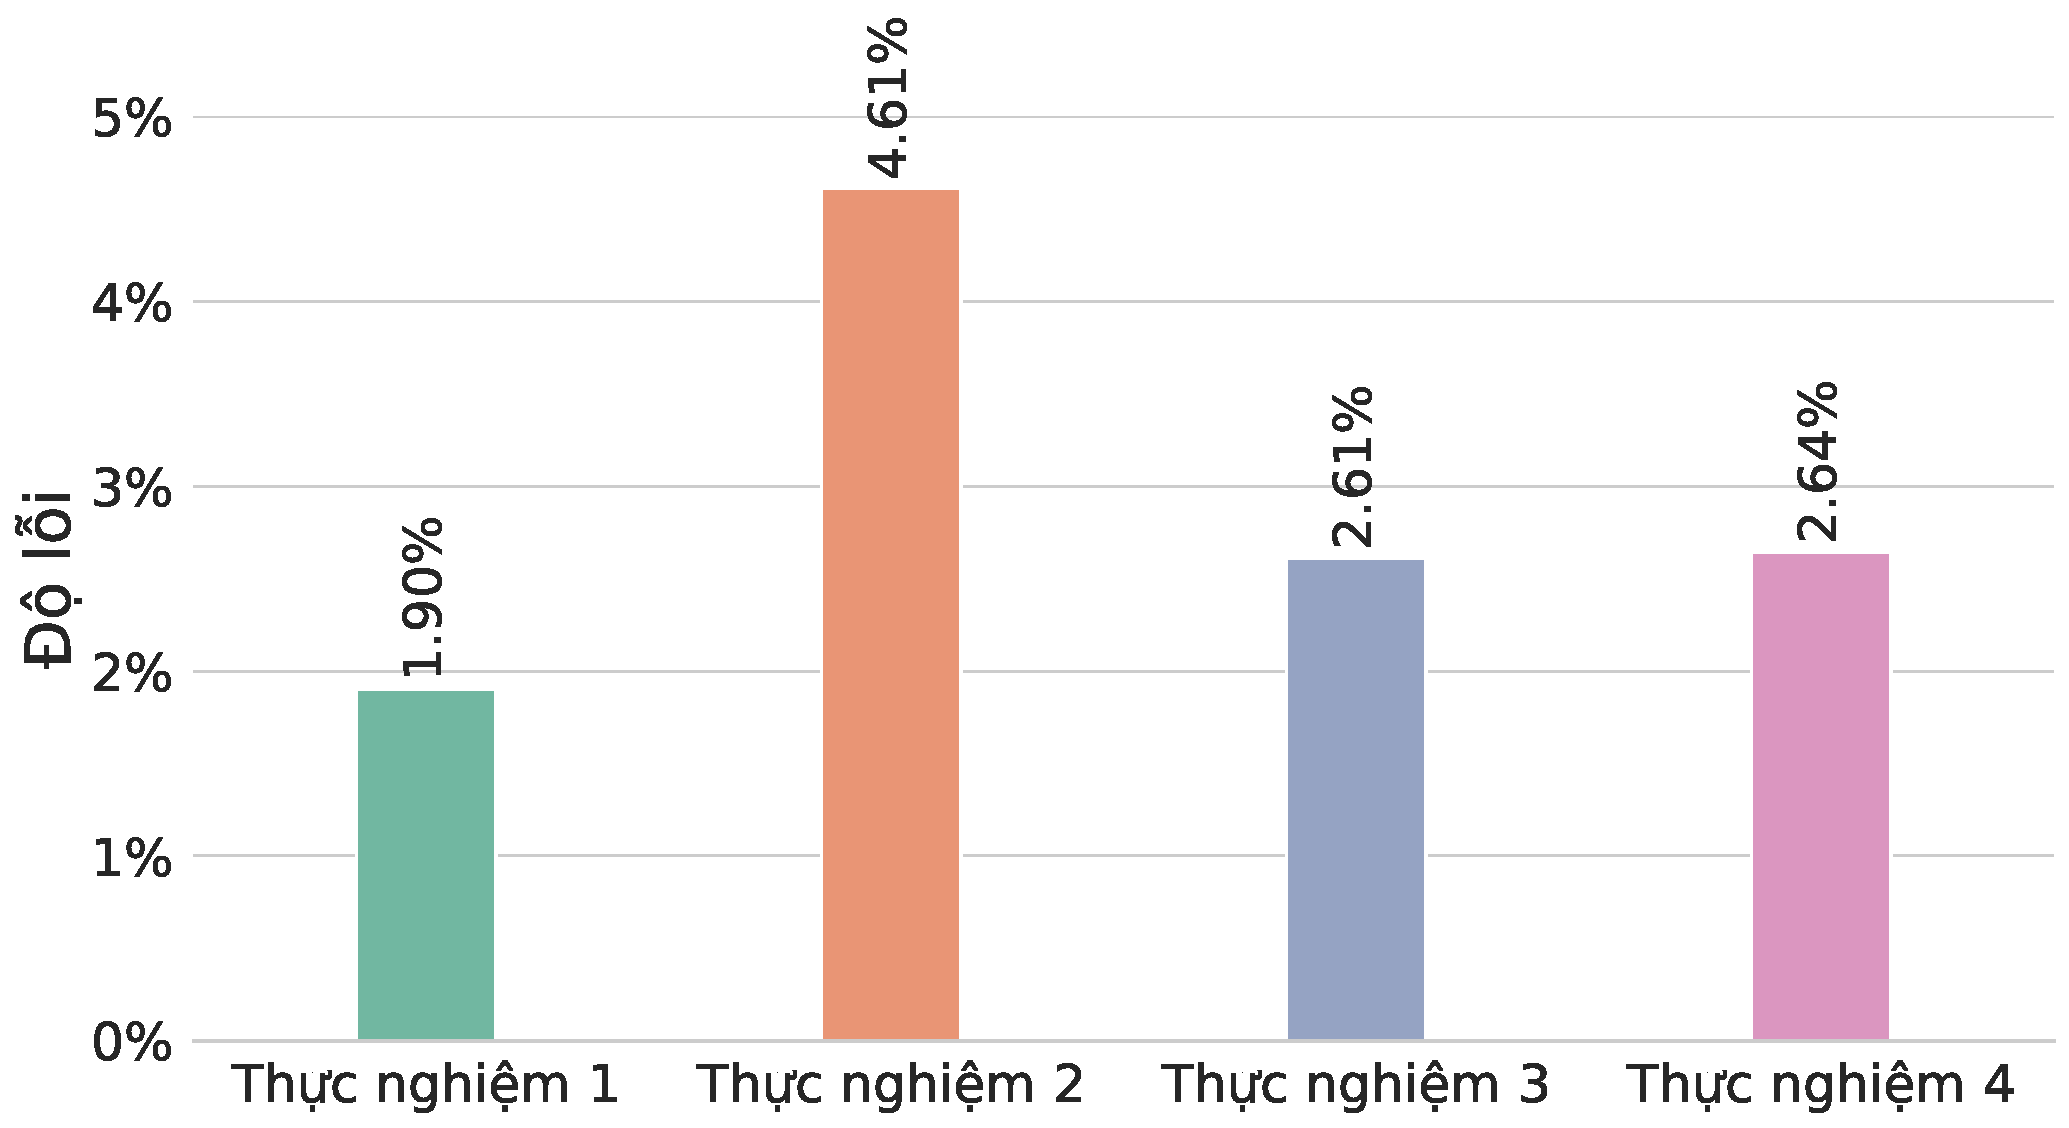
\includegraphics[width=\textwidth]{Figures/sensitive_error_rate.pdf}
    \caption[Minh họa tỷ lệ lỗi trung bình của các thí nghiệm ACO++ với các bộ siêu tham số khác nhau.]{Minh họa tỷ lệ lỗi trung bình từ mỗi thí nghiệm so với kết quả tốt nhất giữa bốn thí nghiệm cho mỗi nhóm trường hợp. Chúng tôi thực hiện 30 lần chạy độc lập cho mỗi trường hợp.}
    \label{fig:ACO++Sensitive}
\end{figure}

Kết quả của những thí nghiệm này được trình bày trong Hình \ref{fig:ACO++Sensitive}. Các thí nghiệm của chúng tôi cho thấy sự biến động đáng kể qua các bộ siêu tham số khác nhau cho thuật toán ACO++. Đặc biệt là sự chênh lệch đáng chú ý được quan sát trong Thí nghiệm 2, nơi việc hoán đổi các bộ tham số dẫn đến sự tăng đáng kể 4,61\% trong tỷ lệ lỗi - hơn gấp đôi con số của Thí nghiệm 1, nơi sử dụng cấu hình tham số cụ thể cho từng trường hợp, mang lại tỷ lệ lỗi chỉ là 1,90\%. Ngược lại, Thí nghiệm 3 và 4 thể hiện tỷ lệ lỗi tương đương khoảng 2,60\%. Các thí nghiệm của chúng tôi ở đây cho thấy sự nhạy cảm của ACO++ đối với các siêu tham số của nó.

\section{Cơ chế thích ứng tốc độ bay hơi pheromone}\label{section:AdaptivePheromoneRate}
Các thuật toán heuristics thường rất nhạy cảm đối với cài đặt tham số và do đó, chúng thiếu tính ổn định để giải quyết mọi cấu hình vấn đề một cách tổng quát. Vấn đề này thường được xử lý bằng cách sử dụng mỗi bộ tham số riêng cho từng trường hợp. Điều này rất tốn thời gian khi ta xem xét đến tính thực tế của thuật toán.

Từ quan điểm này, thì có vẻ như tham số quan trọng nhất đối với các thuật toán dựa trên tối ưu hóa đàn kiến là hệ số bay hơi mùi $\rho$. Hệ số này kiểm soát tốc độ bay hơi của pheromone, ảnh hưởng quyết định đến quá trình hội tụ của thuật toán. Giá trị càng lớn, quá trình hội tụ đến một điểm tối ưu cục bộ càng nhanh. Việc chọn giá trị bay hơi $\rho$ phù hợp phụ thuộc vào bản đồ mà trường hợp thuật toán đang giải.

Công trình về phương pháp AACO-NC \cite{STODOLA2022101056}, một thuật toán cho TSP, đã đề xuất một phương pháp thích ứng tham số tốc độ bay hơi pheromone $\rho$ cho thuật toán dựa trên tối ưu hóa đàn kiến. Ý tưởng của phương pháp này là tham số $\rho$ sẽ không cố định xuyên suốt quá trình thuật toán xử lý. Tham số $\rho$ sẽ thay đổi trong quá trình tối ưu hóa dựa trên thông tin đa dạng của các lời giải sinh ra bởi đàn kiến, thông tin này gọi là entropy. Tại điểm bắt đầu tối ưu hóa, khi mà độ đa dạng của lời giải đàn kiến lớn (giá trị entropy lớn) bởi vì các lời giải hoàn toàn ngẫu nhiên, thì giá trị của tốc độ bay hơi $\rho$ phải lớn để đảm bảo thuật toán hội tụ nhanh. Tuy nhiên, trong quá trình tối ưu hóa, khi mà các lời giải của đàn kiến bắt đầu hội tụ vào một điểm tối ưu cục bộ nào đó, giá trị tốc độ bay hơi $\rho$ nên giảm xuống để mở rộng không gian tìm kiếm.

Giá trị độ đa dạng của các lời giải trong đàn kiến được tính dựa trên công thức Shannon entropy H được trình bày bởi công thức dưới đây.

\begin{equation}\label{eq:AACO-NC:entropy}
    H = -\sum_{i=2}^{n}\sum_{j=1}^{i-1}p_{ij} \cdot \log_2 p_{ij}
\end{equation}

Trong đó $p_{ij}$ là xác suất mà cạnh $E_{ij}$ nối 2 đỉnh $v_i$ và $v_j$ ($i \neq j$) xuất hiện trong bất kỳ lời giải của đàn kiến. Giá trị xác suất này được tính bằng số lần xuất hiện của cạnh trong các lời giải theo công thức sau

\begin{equation}\label{eq:AACO-NC:entropy_prob}
    p_{ij} = \frac{\textit{\# số lần xuất hiện}(E_{ij})}{n \cdot n_{ants}}
\end{equation}

với $\textit{số lần xuất hiện}(E_{ij})$ là số lần cạnh $E_{ij}$ nối 2 đỉnh $v_i$ và $v_j$ xuất hiện trong các lời giải của đàn kiến.

Giá trị giới hạn cực tiểu và cực đại của entropy cho các lời giải của đàn kiến  được tính theo hai công thức \ref{eq:AACO-NC:entropymin} và \ref{eq:AACO-NC:entropymax}.

\begin{equation}\label{eq:AACO-NC:entropymin}
    H_{min} = \log_2 \frac{1}{n}
\end{equation}

\begin{equation}\label{eq:AACO-NC:entropymax}
    H_{min} = \log_2 \frac{1}{n\cdot n_{ants}}
\end{equation}

với n là số lượng đỉnh trong đồ thị (hay số lượng thành phố trong bản đồ); $n_{ants}$ là số lượng lời giải sinh ra bởi đàn kiến.

Tham số tốc độ bay hơi $\rho$ thay đổi trong khoảng giới hạn được gán tại thời điểm bắt đầu thuật toán:
\begin{itemize}
    \item $\rho_{min}$: cận dưới của tham số tốc độ bay hơi ($0 < \rho_{min} \leq \rho_{max}$)
    \item $\rho_{min}$: cận trên của tham số tốc độ bay hơi ($\rho_{min} \leq \rho_{max} < 1$)
\end{itemize}

Giá trị của tham số tốc độ bay hơi pheromone $\rho$ ở mỗi thế hệ được tính theo công thức \ref{eq:AACO-NC:adaptrho}. Công thức này thể hiện tham số $\rho$ phụ thuộc tuyến tính vào giá trị entropy giới hạn.

\begin{equation}\label{eq:AACO-NC:adaptrho}
    \rho = \rho_{\text{min}} + (\rho_{\text{max}} - \rho_{\text{min}}) \cdot \frac{H - H_{\text{min}}}{H_{\text{max}} - H_{\text{min}}}.
\end{equation}

Điểm mạnh của nguyên tắc này là tham số tốc độ bay hơi phản ánh sự tiến triển hiện tại trong quá trình tối ưu hóa. Khi quần thể có xu hướng hội tụ đến một tối ưu cục bộ, tham số cũng được giảm, do đó, pheromone bay hơi chậm hơn với ảnh hưởng của sự hội tụ chậm hơn. Điều này mở rộng không gian tìm kiếm dẫn đến khả năng khám phá một tối ưu cục bộ tốt hơn (hoắc có thể là toàn cục).

\section{Thuật toán tiến hóa CMA-ES}\label{section:bgCMA-ES}
Thuật toán Covariance Matrix Adaptation Evolution Strategy (CMA-ES) là một phương pháp tối ưu hóa tiến hóa được thiết kế để giải quyết các bài toán tối ưu hóa không đạo hàm. Được đề xuất bởi Nikolaus Hansen vào năm 2003 \cite{hansen2003ecj}, CMA-ES đã trở thành một trong những thuật toán quan trọng trong lĩnh vực tối ưu hóa tiến hóa.

CMA-ES kết hợp giữa hai yếu tố chính là ma trận hiệp phương sai (covariance matrix) và chiến lược tiến hóa (evolution strategy). Trong quá trình tối ưu hóa, thuật toán không chỉ tìm kiếm giải pháp tốt mà còn điều chỉnh ma trận hiệp phương sai để thích ứng với cấu trúc hình dạng của không gian tìm kiếm.

\begin{figure}[ht!]
    \centering
    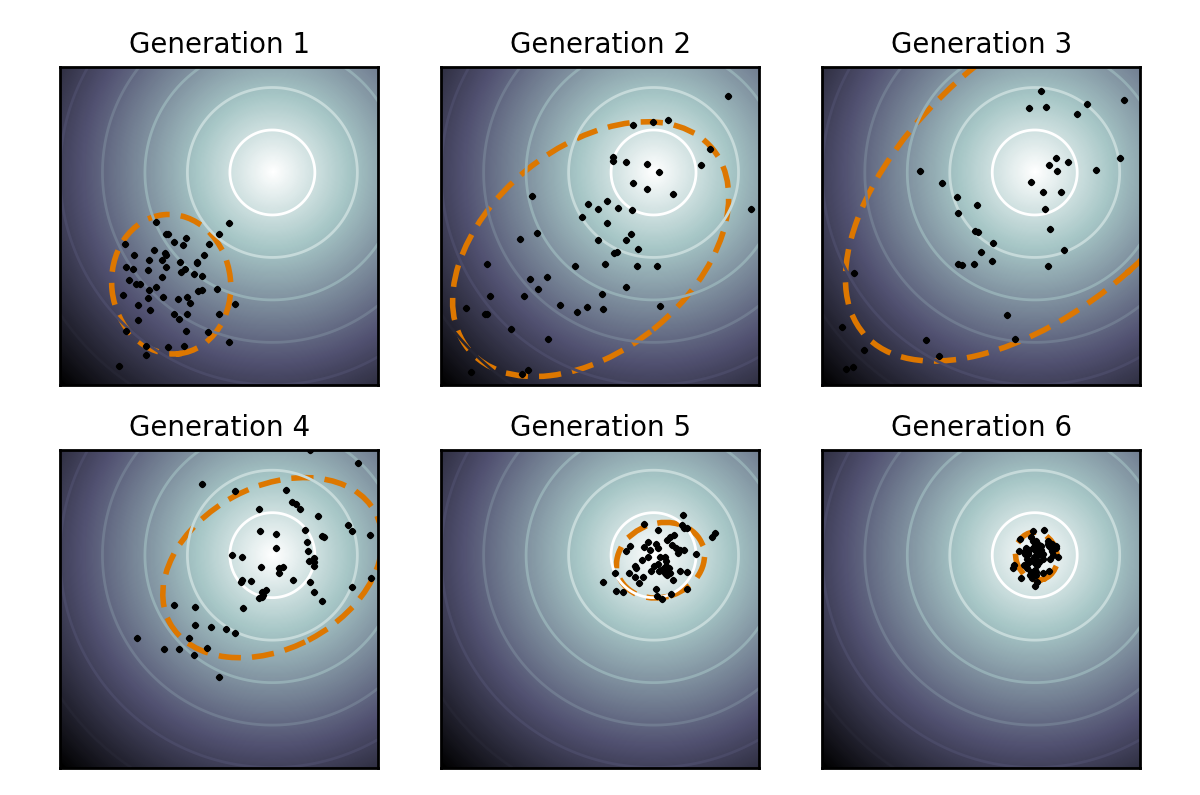
\includegraphics[width=0.85\textwidth]{Figures/Concept_of_directional_optimization_in_CMA-ES_algorithm.png}
    \caption[Minh họa quá trình CMA-ES tối ưu hóa một bài toán 2 chiều đơn giản.]{Minh họa quá trình CMA-ES tối ưu hóa một bài toán 2 chiều đơn giản. Địa hình tối ưu hóa hình cầu được biểu diễn dưới các đường liền. Quần thể được biểu diễn dưới các chấm và phân phối của CMA-ES được biểu diễn bằng đường đứt nét thay đổi qua các thế hệ. Trong bài toán đơn giản này, quần thể tập trung vào cực trị toàn cục chỉ trong vài thế hệ.}
    \label{fig:CMA-ES}
\end{figure}

Một đặc điểm nổi bật của CMA-ES là khả năng xử lý các bài toán tối ưu hóa không đạo hàm và không yêu cầu thông tin đạo hàm của hàm mục tiêu. Điều này làm cho nó trở thành lựa chọn phù hợp trong nhiều ứng dụng thực tế, khi mà việc tính toán đạo hàm có thể khó khăn hoặc tốn kém. Thuật toán thực hiện quá trình tối ưu hóa thông qua việc tạo ra và cập nhật một quần thể các cá thể (solutions) theo thời gian. Các cá thể này được tổ chức thành một phân phối xác suất, và chiến lược tiến hóa được sử dụng để điều chỉnh phân phối này sao cho các cá thể có khả năng sinh sản tốt nhất được ưu tiên. Với sự linh hoạt và hiệu suất của mình, CMA-ES đã được áp dụng rộng rãi trong nhiều lĩnh vực như tối ưu hóa tham số, máy học, và các ứng dụng trong khoa học dữ liệu.

Trong giải thuật \ref{algo:CMAES}, chúng tôi trình bày mã giả tóm tắt đầy đủ cho thuật toán CMA-ES. Giải thuật \ref{algo:CMAES} bắt đầu bằng cách khởi tạo các tham số ở dòng \ref{CMAES-algo:step1} là \ref{CMAES-algo:step2}. Các tham số của thuật toán bao gồm vị trí trung tâm của phân phối m, ma trận hiệp phương sai C, và bước nhảy $\sigma$. Ba tham số này {m, C, $\sigma$} sẽ được tuần tự cập nhật từ dòng \ref{CMAES-algo:step3} đến dòng \ref{CMAES-algo:step11} của thuật toán. Dòng \ref{CMAES-algo:step4} là lấy mẫu một quần thể  từ phân phối chuẩn với vị trí trung tâm m và hiệp phương sai C. Dòng \ref{CMAES-algo:step5} đánh giá các cá thể trong quần thể bằng một hàm hộp đen $f(.)$. Sau đó thuật toán sẽ dùng thông tin đánh giá này để cập nhật vị trí trung tâm m bằng cách lấy tổng $\mu$ cá thể tốt nhất ở dòng \ref{CMAES-algo:step6}, các trọng số được tính bằng log($\mu$/2) - log(i). Ký hiệu $y_{i:\lambda}$ nghĩa là các cá thể tốt nhất từ $y_i$, ..., $y_\lambda$. Ma trận hiệp phương sai được cập nhật ở dòng \ref{CMAES-algo:step10} bao gồm 3 phần: (1) thông tin cũ, (2) cập nhật bậc 1 (được tính bằng sự thay đổi của vị trí trung tâm hay còn gọi là đường tiến hóa $p_c$), và (1) cập nhật bậc $\mu$ được tính bằng các các thể tốt ở quần thể vừa rồi. Tham số bước nhảy được cập nhật ở dòng \ref{CMAES-algo:step8} dựa trên đường tiến hóa liên hợp $p_\sigma$. Mục tiêu của nó là tăng tốc tốc độ hội tụ vào cực trị, trong khi ngăn chặn việc hội tụ sớm. Các tham số khác bao gồm: $\mu_w$ là giá trị chọn hiệu quả phương sai, các tham số tốc độ học $c_1$, $c_c$, $c_\sigma$, và $d_\sigma$ là giá trị làm mượt cho $\sigma$. Các thông số của các tham số này được nghiên cứu kỹ lưỡng và thảo luận sâu trong \cite{hansen2023cma}. Điều kiện để kết thúc có thể được cài đặt nhiều cách khác nhau tùy thuộc vào không gian tìm kiếm, hoặc hàm thích nghi.

\begin{algorithm}
\caption{Thuật toán CMA-ES}
\label{algo:CMAES}
khởi tạo $\mathbf{m} \in \Re^n, \sigma \in \Re^{+}, \lambda, \mu$ \; \label{CMAES-algo:step1}
khởi tạo $\mathbf{C}=\mathbf{I}, \mathbf{p}_c=\mathbf{0}, \mathbf{p}_\sigma=\mathbf{0}$ \;\label{CMAES-algo:step2}
\Repeat{điều kiện dừng được thỏa mãn}{ \label{CMAES-algo:step3} 
lấy mẫu: $\theta_i=\mathbf{m}+\sigma \mathbf{y}_i, \mathbf{y}_i \sim \mathcal{N}(\mathbf{0}, \mathbf{C}), i=1, \ldots, \lambda$ \; \label{CMAES-algo:step4} 
đánh giá: $f\left(\theta_i\right), i=1, \ldots, \lambda$\; \label{CMAES-algo:step5} 
\tcp{cập nhật giá trị trung bình}
$\mathbf{m} \leftarrow \mathbf{m}+\sigma \overline{\mathbf{y}}$, với $\overline{\mathbf{y}}=\sum_1^\mu w_i \mathbf{y}_{i: \lambda}$\; \label{CMAES-algo:step6} 
\tcp{cập nhật bước nhảy}
$\mathbf{p}_\sigma \leftarrow\left(1-c_\sigma\right) \mathbf{p}_\sigma+\sqrt{c_\sigma\left(2-c_\sigma\right) \mu_w} \mathbf{C}^{-\frac{1}{2}} \overline{\mathbf{y}}$\; \label{CMAES-algo:step7} 
$\sigma \leftarrow \sigma \exp \left(\frac{c_\sigma}{d_\sigma}\left(\frac{\left\|\mathbf{p}_\sigma\right\|}{\mathbb{E}\|\mathcal{N}(\mathbf{0}, \mathbf{I})\|}-1\right)\right)$ \;\label{CMAES-algo:step8} 
\tcp{cập nhật ma trận hiệp phương sai}
$\mathbf{p}_c \leftarrow\left(1-c_c\right) \mathbf{p}_c+\sqrt{c_c\left(2-c_c\right) \mu_w} \overline{\mathbf{y}}$\;\label{CMAES-algo:step9} 
$\mathbf{C} \leftarrow\left(1-c_1-c_\mu\right) \mathbf{C}+c_1 \mathbf{p}_c \mathbf{p}_c^{\top}+c_\mu \sum_1^\mu w_i \mathbf{y}_{i: \lambda} \mathbf{y}_{i: \lambda}^{\top}$\;\label{CMAES-algo:step10} 
}\label{CMAES-algo:step11}
\end{algorithm}

\section{Kỹ thuật cài đặt tham số}\label{section:parametersetting}
Với các thuật toán heurisitic như thuật toán tối ưu hóa đàn kiến và thuật toán tiến hóa thì hiệu suất của các thuật toán này phụ thuộc phần lớn vào các tham số của chúng. Ở khóa luận này chúng tôi đặt trọng tâm vào việc tự động thích ứng các tham số của thuật toán ACO++, một thuật toán heuristic. Để dễ dàng nắm bắt được những kỹ thuật mà chúng tôi trình bày, ở phần này chúng tôi trình bày kiến thức cơ bản về các kỹ thuật cài đặt siêu tham số khác nhau cho một thuật toán heuristic.

Chúng tôi xem rằng có hai loại cài đặt tham số chính là điều chỉnh siêu tham số (parameter tuning) và kiểm soát siêu tham số (parameter control) \cite{771166}. Với điều chỉnh siêu tham số, là phương pháp cài đặt tham số thường xuyên được sử dụng, thì quá trình tìm ra các giá trị tham số tốt được thực hiện trước khi thuật toán chạy và sau đó dùng những tham số được tìm thấy cho thuật toán và không thay đổi trong quá trình chạy. Phương pháp điều chỉnh siêu tham số là hướng tiếp cận điển hình khi thiết kế thuật toán. Quá trình điều chỉnh được thực hiện bằng cách thử nghiệm nhiều giá trị tham số và chọn thủ công ra bộ tham số có kết quả tốt nhất. Tuy nhiên, với phương pháp này thì số lượng tham số và khoảng giá trị của chúng có thể dẫn đến quá trình điều chỉnh siêu tham số này rất tốn thời gian. Và phương pháp này có thể dẫn đến hiệu suất tổng quát thuật toán không tốt nếu các tham số này chỉ được thử nghiệm trên một tập trường hợp nhất định.

Phương pháp kiểm soát tham số là phương pháp đối nghịch với phương pháp điều chỉnh tham số trên. Các tham số sẽ được gán các giá trị khởi tạo khi bắt đầu thuật toán và thay đổi trong quá trình thuật toán chạy. Phương pháp này có thể giải quyết được vấn đề hiệu suất tổng quát của thuật toán bởi vì các tham số sẽ thay đổi giá trị theo từng trường hợp trong quá trình chạy của thuật toán. Hơn nữa với phương pháp này, nếu ta thiết kế nó đủ thông minh, nó có thể không cần tới quá trình điều chỉnh tham số thủ công tốn thời gian mà vẫn tìm ra tham số tốt cho thuật toán. Ở kỹ thuật kiểm soát tham số này, các tác giả của công trình \cite{771166} đã phân loại ra ba cơ chế con dựa trên cách hoạt động của chúng bao gồm cơ chế xác định, cơ chế thích ứng, cơ chế tự thích ứng. Hình \ref{fig:parameterSettingTaxonomy} Minh họa phân loại các kỹ thuật cài đặt tham số.

\begin{figure}[ht!]
    \centering
    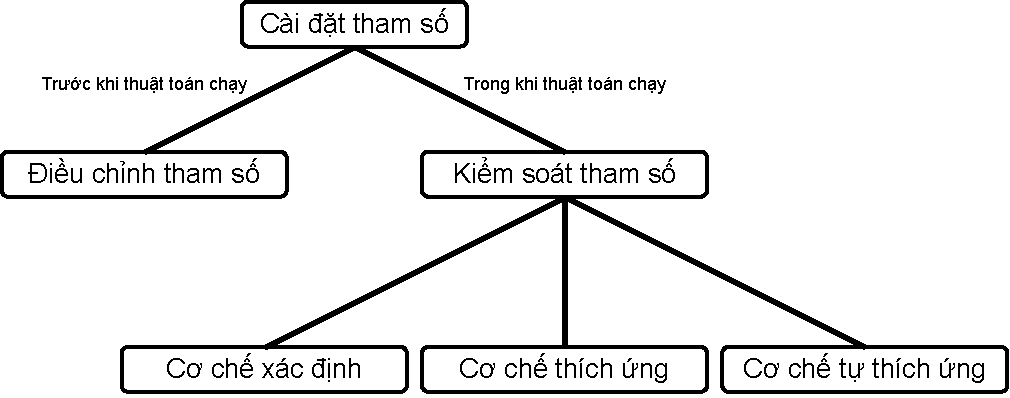
\includegraphics[width=0.8\textwidth]{Figures/Parameter setting.drawio.pdf}
    \caption[Minh họa phân loại các kỹ thuật cài đặt tham số.]{Minh họa phân loại các kỹ thuật cài đặt tham số}
    \label{fig:parameterSettingTaxonomy}
\end{figure}

Cơ chế kiểm soát tham số xác định là cơ chế mà khi giá trị của một tham số được thay đổi bởi một quy tắc xác định. Quy tắc này điều chỉnh tham số  theo một cách cố định, quy tắc xác định được định nghĩa sẵn (tức là được định nghĩa thủ công) mà không sử dụng bất kỳ phản hồi nào từ quá trình tìm kiếm. Thông thường, thì cơ chế này giống như cơ chế lập lịch mà tham số biến đổi theo thời gian.

Cơ chế kiểm soát tham số thích ứng là cơ chế mà khi có một hình thức phản hồi từ quá trình tìm kiếm được sử dụng làm đầu vào cho một một thủ tục để điều chỉnh tham số. Việc gán giá trị cho tham số  có thể dựa trên chất lượng của các lời giải được tìm ra bởi thuật toán. Ví dụ cho cơ chế này là cơ chế thích ứng tốc độ bay hơi pheromone chúng tôi đã trình bày ở phần \ref{section:AdaptivePheromoneRate}, tham số tốc độ bay hơi của thuật toán được điều chỉnh dựa trên chất lượng của các lời giải mà thuật toán tìm được ở vòng lặp hiện tại. 

Cuối cùng là cơ chế kiểm kiểm soát tự thích ứng, ví dụ điển hình cho cơ chế này là thuật toán CMA-ES mà chúng tôi đã trình bày ở phần \ref{section:CMAES}. Ở đây, các tham số cần được điều chỉnh được mã hóa vào các cá thể và trải qua quá trình đột biến và tái kết hợp. Các giá trị tốt hơn của các tham số được mã hóa này dẫn đến các cá thể tốt hơn, từ đó có khả năng cao hơn để sống sót, tạo ra con cái và do đó lan truyền những giá trị tham số tốt hơn này. Điều này là sự phân biệt quan trọng giữa các cơ chế thích ứng và cơ chế tự thích ứng: trong trường hợp tự thích ứng, các cơ chế cho việc gán điểm và cập nhật các tham số chiến lược khác nhau là hoàn toàn ngụ ý, tức là chúng là các toán tử lựa chọn và biến đổi của chu kỳ tiến hóa chính nó.

\section{Phương pháp phân cụm thứ bậc}\label{section:bgClusterTree}

Phân cụm thứ bậc là một kỹ thuật phân cụm nhằm xây dựng một cấu trúc cây của các cụm hay cây cụm thứ bậc. Cây cụm thứ bậc mang cấu trúc dữ liệu cây với mỗi nút là một cụm. Trong đó, tập điểm dữ liệu của một nút con là một phần trong tập điểm dữ liệu của nút ba mẹ. Phân cụm thứ bậc có thể giúp biểu hiện cấu trúc phân cấp tự nhiên có trong các điểm dữ liệu.

Phân cụm thứ bậc có hai loại là phân cụm phân chia (divisive clustering) và phân cụm hội tụ (agglomerative clustering) \cite{shetty2021hierarchical}. Phân chia là một phương pháp từ trên xuống bắt đầu với một cụm bao gồm tất cả các điểm dữ liệu. Nó chia các cụm thành các cụm con một cách tuần tự cho đến khi bản thân cụm là một điểm dữ liệu. Ngược lại, phân cụm hội tụ là một phương pháp từ dưới lên bắt đầu với mỗi điểm dữ liệu như một cụm đơn và sau đó hợp nhất các cụm gần nhau để tạo ra các cụm lớn hơn cho đến khi chỉ còn lại một cụm chứa tất cả các điểm dữ liệu. Cách phân chia hoặc hợp nhất các cụm phụ thuộc vào ứng dụng và đặc tính của dữ liệu. Do đó, phân cụm thứ bậc có nhiều biến thể và độ phức tạp không gian, thời gian khác nhau \cite{murtagh2012algorithms, murtagh2017algorithms}.
